% Metódy inžinierskej práce

\documentclass[10pt,twoside,slovak,a4paper]{article}

\usepackage[slovak]{babel}
%\usepackage[T1]{fontenc}
\usepackage[IL2]{fontenc} % lepšia sadzba písmena Ľ než v T1
\usepackage[utf8]{inputenc}
\usepackage{graphicx}
\usepackage{url} % príkaz \url na formátovanie URL
\usepackage{hyperref} % odkazy v texte budú aktívne (pri niektorých triedach dokumentov spôsobuje posun textu)

\usepackage{cite}
%\usepackage{times}

\pagestyle{headings}

\title{Pecomendation system: eBay\thanks{Semestrálny projekt v predmete Metódy inžinierskej práce, ak. rok 2015/16, vedenie: Meno Priezvisko}} % meno a priezvisko vyučujúceho na cvičeniach

\author{Kuchinka Ivan\\[2pt]
	{\small Slovenská technická univerzita v Bratislave}\\
	{\small Fakulta informatiky a informačných technológií}\\
	{\small \texttt{...@stuba.sk}}
	}

\date{\small 30. september 2015} % upravte



\begin{document}

\maketitle

\begin{abstract}
\ldots
\end{abstract}



\section{Úvod}

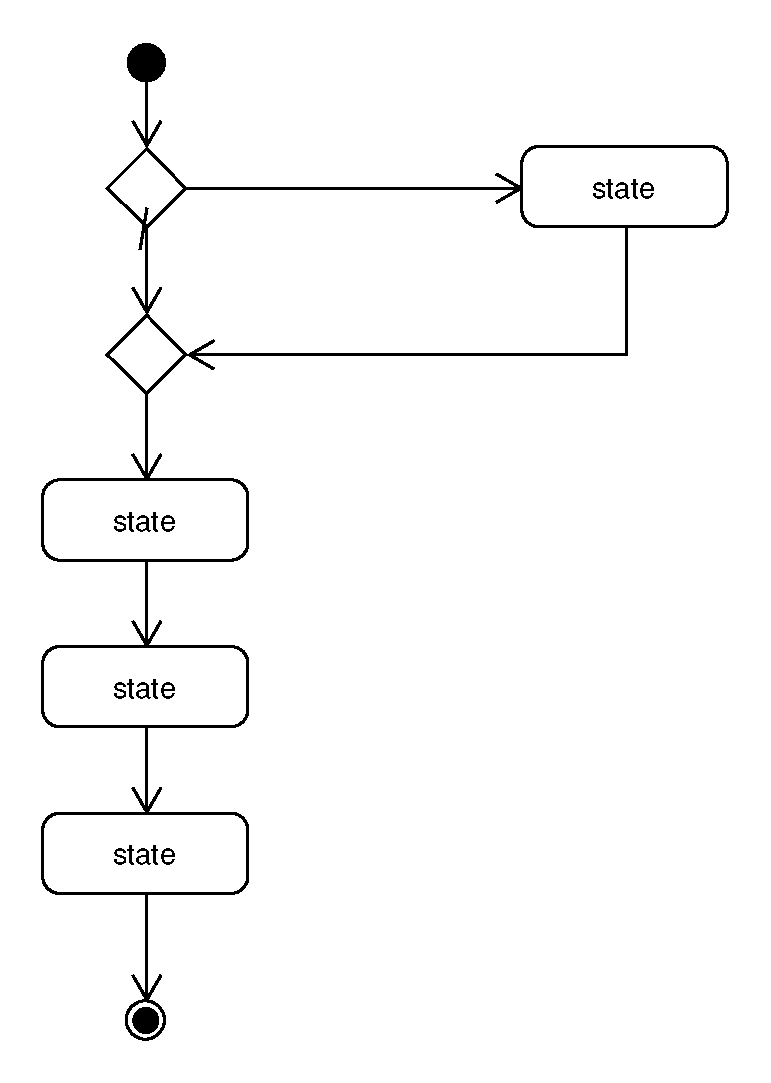
\includegraphics[width=1\textwidth]{img2.pdf}

\section{Nejaká časť} \label{nejaka}


\begin{figure*}[tbh]
\centering

\caption{Rozhodujúci argument.}
\label{f:rozhod}
\end{figure*}



\section{Iná časť} \cite{PLP-Framework}\label{ina}


\section{Ešte dôležitejšia časť} \label{dolezitejsia}




\section{Záver} \label{zaver} % prípadne iný variant názvu



%\acknowledgement{Ak niekomu chcete poďakovať\ldots}


% týmto sa generuje zoznam literatúry z obsahu súboru literatura.bib podľa toho, na čo sa v článku odkazujete
\bibliography{literatura}
\bibliographystyle{plain} % prípadne alpha, abbrv alebo hociktorý iný
\end{document}
